\documentclass{standalone}

\usepackage{xcolor}

\definecolor{myblue}{HTML}{377EB8}
\definecolor{myred}{HTML}{E41A1C}
\definecolor{myviolet}{HTML}{984EA3}
\definecolor{myteal}{HTML}{008B8B}

\usepackage{tikz}
\usepackage{pgfplots}
\pgfplotsset{compat=newest}

\usepackage{lmodern}
\SetSymbolFont{letters}{bold}{OML}{cmbr}{bx}{it}
\renewcommand{\familydefault}{\sfdefault}

\usepackage{sansmathfonts}

\begin{document}
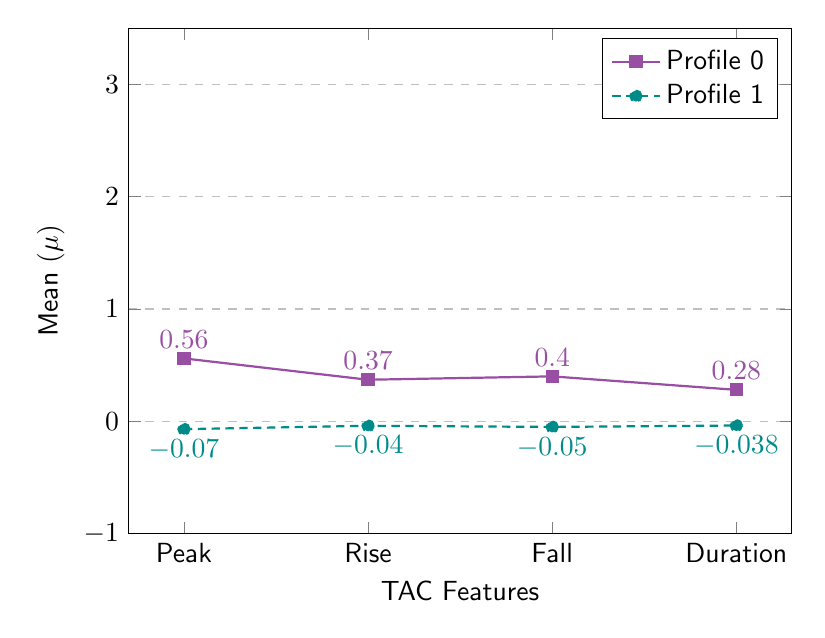
\begin{tikzpicture}
	\begin{axis}[
			xlabel={TAC Features},
			ylabel={Mean $\left( \mu \right)$},
			ymin=-1,
			ymax=3.50,
			xtick=data,
			xticklabels={Peak, Rise, Fall, Duration},
			width=10cm,
			height=8cm,
			nodes near coords,
			nodes near coords={
				\pgfmathprintnumber[fixed, precision=3]{\pgfplotspointmeta}
			},
			ymajorgrids=true,
			grid style=dashed,
		]
		\addplot[myviolet, mark=square*, solid, thick] coordinates {
			(1, 0.560)
			(2, 0.370)
			(3, 0.400)
			(4, 0.280)
		};
		\addplot[myteal, mark=oplus*, densely dashed, thick] coordinates {
			(1, -0.070)
			(2, -0.040)
			(3, -0.050)
			(4, -0.0375)        
		};
		% \draw[lightgray,dashed] (0,0) -- (5,0);
		\legend{Profile 0,Profile 1}
	\end{axis}
\end{tikzpicture}
\end{document}
